\documentclass[12pt,letterpaper]{article}
%NOTE: This report format is 

\newcommand{\reporttitle}{Calculated Vulnerability: An Ethical Analysis of the Dual\_EC\_DRBG Backdoor}
\newcommand{\reportauthorOne}{Qabas Alkaissi}
\newcommand{\cidOne}{20210786}
\newcommand{\reportauthorTwo}{Leen Abu Jamous}
\newcommand{\cidTwp}{20241153}
\newcommand{\reporttype}{Coursework}
\newcommand{\reportauthorThree}{Eng. Fadia El Issa}
\bibliographystyle{plain}

% include files that load packages and define macros
\input{includes} % various packages needed for maths etc.
\input{notation} % short-hand notation and macros

\usepackage{xcolor}
\usepackage{listings}
\usepackage[margin=1in]{geometry}
\usepackage[table]{xcolor}
\usepackage{array}
\usepackage{subcaption}  
\usepackage{float}

\definecolor{codegreen}{rgb}{0,0.6,0}
\definecolor{codegray}{rgb}{0.5,0.5,0.5}
\definecolor{codepurple}{rgb}{0.58,0,0.82}
\definecolor{codenumber}{rgb}{0.7,0.1,0.1}
\definecolor{registerblue}{rgb}{0.2,0.2,0.8}
\definecolor{instrblack}{rgb}{0.1,0.1,0.1}
\definecolor{backcolour}{rgb}{0.97,0.97,0.97}
\definecolor{table}{rgb}{0.90,0.90,0.90}

\newcolumntype{P}[1]{>{\centering\arraybackslash}p{#1}}

%%%%%%%%%%%%%%%%%%%%%%%%%%%%

\begin{document}
% front page
\input{titlepage}


%%%%%%%%%%%%%%%%%%%%%%%%%%% table of content
%If a table of content is needed, simply uncomment the following lines
\tableofcontents
\newpage

%%%%%%%%%%%%%%%%%%%%%%%%%%%% Main document 
\section{Introduction}

In the modern digital landscape, the security of every encrypted transaction, from banking to national defense, relies on a single, critical foundation: the generation of random numbers.   If the random-bit generator (RBG) used to create cryptographic keys is predictable, the entire security protocol collapses. \\ \\This report analyzes the case of the Dual\_EC\_DRBG (Dual Elliptic Curve Deterministic Random Bit Generator), a standard adopted by the U.S. National Institute of Standards and Technology (NIST) in 2006. While NIST is tasked with promoting innovation and setting technical standards, the Dual\_EC\_DRBG algorithm became the center of a massive ethical controversy. \\ \\ Allegations surfaced that the National Security Agency (NSA) had engineered a mathematical "backdoor" into the algorithm and struck a deal with security vendor RSA to make it the default in their products. In April 2014, NIST officially withdrew support for the algorithm, rendering it non-compliant. This case study examines how a compromised engineering standard violates the public trust and the fundamental canons of engineering ethics.

\section{Conceptual Background}
\subsection{Random Bit Generators}
Deterministic Random Bit Generators (DRBGs), often referred to as Pseudorandom Number Generators (PRNGs), are cryptographic algorithms that expand a relatively short, high-entropy secret value, known as the seed ($s$), into a long sequence of bits that are computationally indistinguishable from truly random data.
\\ \\
As standardized in NIST SP 800-90A \cite{Barker2015}, a DRBG operates by maintaining an internal state which is updated deterministically using a cryptographic primitive, such as a block cipher (as seen in CTR\_DRBG using AES) or a hash function (as in Hash\_DRBG or HMAC\_DRBG).

\begin{figure}
    \centering
    \includegraphics[width=0.9\linewidth]{figures/Block-cipher_-removebg-preview.png}
    \caption{Block Cipher for CTR\_DRBG}
    \label{fig:placeholder}
\end{figure}

\subsection{Elliptic Curves}

Elliptic curves are mathematical objects defined by algebraic equations of the form
\[
y^2 = x^3 + ax + b,
\]
where the parameters \(a\) and \(b\) are chosen such that the curve has no singularities. Although these curves appear geometric, their most important property is algebraic: points on an elliptic curve can be combined using a well-defined addition operation, forming an abelian group \cite{washington2008elliptic}.

\begin{figure}[H]
\centering
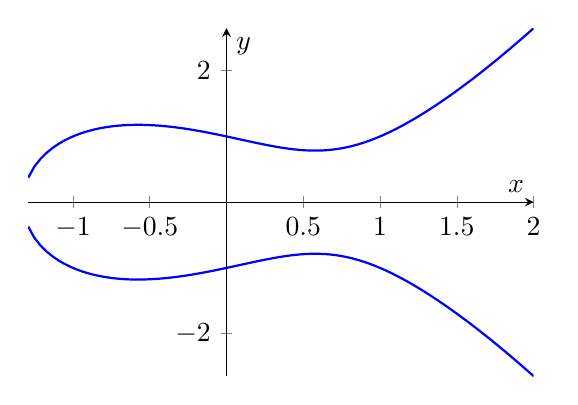
\begin{tikzpicture}
\begin{axis}[
    axis lines=middle,
    xlabel={$x$},
    ylabel={$y$},
    samples=100,
    domain=-2:2,
    width=8cm,
    height=6cm
]
    \addplot[blue, thick, domain=-1.879:2] {sqrt(x^3 - x + 1)};
    \addplot[blue, thick, domain=-1.879:2] {-sqrt(x^3 - x + 1)};
\end{axis}
\end{tikzpicture}
\caption{Example of an elliptic curve defined by $y^2 = x^3 - x + 1$.}
\label{fig:elliptic_curve}
\end{figure}



This group structure enables the use of elliptic curves in public-key cryptography. Elliptic Curve Cryptography (ECC) relies on the difficulty of the \textit{Elliptic Curve Discrete Logarithm Problem (ECDLP)}, which involves determining an unknown scalar given two points on the curve. This problem is considered computationally infeasible for properly chosen curves and parameters \cite{koblitz1987elliptic}.

A key advantage of ECC is efficiency. Elliptic-curve-based systems provide the same level of security as traditional cryptographic schemes, such as RSA, but with significantly smaller key sizes. This results in faster computations, reduced memory usage, and lower power consumption, making ECC especially suitable for constrained environments like embedded systems and mobile devices \cite{nist2018ecc}.

Because of these benefits, elliptic curves are widely used in modern cryptographic protocols, including digital signatures (ECDSA), key exchange (ECDH), and random number generation mechanisms.

\subsection{Dual\_EC\_DRBG}

Dual\_EC\_DRBG is a deterministic random bit generator standardized by NIST as part of SP 800-90A. Unlike most random number generators, Dual\_EC\_DRBG is based on elliptic curve point multiplication rather than hash functions or block ciphers \cite{nist2015sp80090a}.

The generator operates by repeatedly multiplying secret internal state values with fixed elliptic curve points and extracting output bits from the resulting coordinates. While mathematically sound in principle, this design introduces a critical dependency on the choice of public curve parameters.

\vspace{0.45cm}

\begin{tikzpicture}[
    % Tighter node distance to prevent margin bleeding
    node distance=1.5cm and 1.5cm,
    font=\sffamily,
    >=Latex,
    block/.style={
        draw, 
        rectangle, 
        minimum height=0.9cm, 
        minimum width=1.6cm, 
        align=center,
        font=\bfseries\small
    },
    sum/.style={
        draw, 
        circle, 
        inner sep=0pt, 
        minimum size=0.5cm,
        node contents={\large $+$}
    },
    switch/.style={
        draw, 
        circle, 
        minimum size=0.8cm,
        inner sep=0pt
    },
    label_text/.style={
        font=\scriptsize, 
        align=center
    }
]

    % --- 1. Central Adder ---
    \node (adder) [sum];

    % --- 2. Switches (Positioned closer to Adder) ---
    % Adjusted coordinates to pull them inward
    \node (sw_top) [switch, above left=0.8cm and 0.1cm of adder] {};
    \node (sw_bot) [switch, below left=0.8cm and 0.1cm of adder] {};

    % Internal Switch Levers (Visual fix)
    % Top switch (points up to feedback by default or left to seed)
    \draw[thick] (sw_top.center) -- (sw_top.south); 
    % Bottom switch (points left)
    \draw[thick] (sw_bot.center) -- (sw_bot.north);

    % --- 3. Main Processing Chain (Right Side) ---
    \node (phi1) [block, right=1.2cm of adder] {$\varphi(x(t*P))$};
    \node (phi2) [block, right=1cm of phi1] {$\varphi(x(s*Q))$};
    \node (extract) [block, right=0.8cm of phi2, minimum height=1cm] {Extract\\Bits};

    % Parameters P and Q
    \node (P) [below=0.5cm of phi1] {\textbf{P}};
    \node (Q) [below=0.5cm of phi2] {\textbf{Q}};

    % --- 4. Inputs (Left Side - Tightened) ---
    
    % Seed Input: Positioned closer to switch
    \node (seed) [left=0.6cm of sw_top, font=\bfseries] {seed};
    
    % Optional Input: Right aligned text to save left-margin space
    \node (opt_input) [left=0.6cm of sw_bot, align=right, font=\bfseries\small] {[Optional]\\add. input};
    
    % The '0' input
    \node (zero) [below left=0.1cm and 0.6cm of sw_bot, font=\bfseries] {0};

    % --- 5. Connections ---

    % Top Switch Connections
    \draw[->] (seed) -- (sw_top.west);
    \draw[->] (sw_top.south) -- (adder.north);
    
    % Annotation for Seed (moved closer)
    \node [below=0.1cm of seed, label_text, align=right, anchor=north] {Instant. or\\reseed only};

    % Bottom Switch Connections
    \draw[->] (opt_input.east) -- (sw_bot.west);
    \draw[->] (zero.east) -- (sw_bot.225); % Connects to bottom-left of circle
    \draw[->] (sw_bot.north) -- (adder.south);

    % Annotation for Null Input
    \node [below=0.4cm of opt_input, label_text, align=right] {If additional\\input = Null};

    % Adder to Phi1
    \draw[->] (adder.east) -- node[above, font=\small] {\textbf{t}} (phi1.west);

    % P and Q lines
    \draw[->] (P) -- (phi1.south);
    \draw[->] (Q) -- (phi2.south);

    % Chain connections
    \draw[->] (phi1.east) -- node[above, font=\small] {\textbf{s}} (phi2.west);
    \draw[->] (phi2.east) -- node[above, font=\small] {\textbf{r}} (extract.west);

    % Output
    \draw[->] (extract.south) -- ++(0,-0.6) node[below, align=center, font=\bfseries\small] {Pseudorandom\\Bits};

    % --- 6. Feedback Loop ---
    % Drawn neatly to go back to the top switch
    \draw[->] ($(phi1.east)+(0.3,0)$) |- ++(0, 1.2) -| (sw_top.north);

\end{tikzpicture}

In 2007, Shumow and Ferguson demonstrated that if a specific mathematical relationship exists between the standardized elliptic curve points, an entity aware of this relationship could predict future outputs of the generator \cite{shumow2007dualec}. This effectively constitutes a potential cryptographic backdoor, allowing attackers to compromise systems relying on Dual\_EC\_DRBG for randomness.

Although no public proof exists that such a backdoor was intentionally inserted, the lack of transparency surrounding parameter selection raised serious ethical concerns. As a result, Dual\_EC\_DRBG was widely criticized and eventually removed from recommended use, highlighting the importance of trust, openness, and ethical responsibility in cryptographic standardization.


\section{Problem Statement}
To fully analyze this case, we must first dissect the problem into its factual, conceptual, and moral dimensions.

\subsection{Factual Issues}
The case study concerns the controversy surrounding Dual\_EC\_DRBG, a deterministic random bit generator standardized by the National Institute of Standards and Technology (NIST) in Special Publication 800--90A. Dual\_EC\_DRBG was designed to generate cryptographically secure random numbers using elliptic curve cryptography, a fundamental component in modern security protocols. Random number generators are critical because they underpin key generation, nonces, initialization vectors, and other security mechanisms; therefore, any weakness in their design has potentially widespread consequences. The controversy emerged when media reports alleged that the U.S. National Security Agency (NSA) had influenced the inclusion and promotion of Dual\_EC\_DRBG within the NIST standard, and that RSA Security had allegedly accepted incentives to make Dual\_EC the default random number generator in its cryptographic products, an allegation that RSA later denied.


From a technical perspective, Dual\_EC\_DRBG operates by repeatedly performing integer–point multiplication on an elliptic curve using two publicly specified points, denoted P and Q. In each iteration, the internal state is updated through multiplication by point P, while the output is derived by multiplying an intermediate value by point Q and extracting the x--coordinate of the resulting elliptic curve point. Importantly, the algorithm truncates the least significant 16 bits of this x--coordinate before producing the final output. Although truncation is typically used to improve security, in this case it plays a key role in the vulnerability described in the study.


The alleged vulnerability arises from the possibility that there exists a secret numerical relationship between the two public points such that $P = eQ$, where e is a secret scalar. If an entity knows this scalar, it becomes theoretically possible to reconstruct the internal state of the generator from its output. The study explains that an attacker who observes the truncated output could brute--force the missing 16 bits, test which candidates lie on the elliptic curve, and then use the secret relationship to predict future outputs. This prediction capability is especially dangerous if the generator produces public random values before being used to derive secret cryptographic keys, as it would drastically reduce the key search space and undermine security guarantees. While it cannot be proven that such a secret relationship was intentionally embedded, the fact that it could exist is central to the ethical and security concerns raised by the case.


The implications of this vulnerability are global rather than localized. Because 

Dual\_EC\_DRBG was standardized by NIST, it gained credibility and was adopted or considered for adoption in commercial and governmental systems. As a result, any weakness in the algorithm could affect a wide range of systems relying on standardized cryptographic primitives. In response to mounting criticism and loss of confidence, NIST announced in April 2014 that it was withdrawing support for Dual\_EC\_DRBG, rendering implementations of the algorithm non-compliant with current standards. The case study concludes that the algorithm was effectively discredited, arguing that it is implausible that the designers were unaware of the vulnerability or that they failed to anticipate its eventual discovery.

\subsection{Conceptual Issues}
At the conceptual level, the case raises fundamental questions about the meaning of randomness in cryptographic systems. In everyday language, randomness refers to unpredictability, but in cryptography it has a much stricter definition. Randomness must be computationally unpredictable to any adversary, as even partial predictability can compromise security. The case study emphasizes that random-bit generation is the foundation of nearly every security protocol, meaning that weaknesses in randomness propagate upward to encryption schemes, authentication mechanisms, and secure communications as a whole. Thus, randomness is not a peripheral technical feature but a core security requirement.

Another important concept highlighted in this case is standardization. NIST plays a central role in defining cryptographic standards that are widely adopted by industry and government. When an algorithm becomes part of a NIST standard, it gains institutional legitimacy and is often assumed to be trustworthy without independent scrutiny by end users. This case demonstrates that standardization amplifies both trust and risk: while standards promote interoperability and consistency, they also create systemic vulnerabilities if a flawed or controversial algorithm is included. As such, standardization carries ethical weight, not merely technical authority, because the consequences of a poor design choice are distributed across a vast user base.

The conceptual integrity of parameter selection is also central to the Dual\_EC\_DRBG controversy. Although the mathematical operations used in the algorithm rely on well-understood cryptographic assumptions, the security of the design depends critically on how the elliptic curve points P and Q were chosen. The potential existence of a secret relationship between these points introduces a trust problem rather than a purely mathematical one. Even if the underlying cryptography is sound, the lack of transparency in parameter generation undermines confidence in the algorithm. This highlights a broader conceptual issue in cryptography: security depends not only on strong mathematics but also on transparent, verifiable processes.

\subsection{Moral Issues}
The moral dimension of this case revolves primarily around conflict of interest, deception versus national security, and public trust. Allegations that the NSA may have influenced the design or promotion of Dual\_EC\_DRBG raise concerns about whether national intelligence objectives conflicted with the broader public interest in secure cryptographic standards. Even though such allegations were denied, the mere possibility of undue influence introduces ethical tension between state surveillance goals and the responsibility to protect global digital security. Standards bodies and vendors occupy positions of trust, and any perception that standards are shaped by hidden agendas damages their moral legitimacy.

A closely related moral issue is the ethical boundary between deception and national security. If a cryptographic standard were intentionally designed to allow selective access by a privileged party, this would constitute deception toward users who rely on the standard for confidentiality and safety. Some might argue that such measures could be justified in the name of national security; however, this case illustrates the ethical cost of that argument. Weakening widely used cryptographic systems does not only affect adversaries but also endangers ordinary users, businesses, and critical infrastructure. From an ethical standpoint, intentionally embedding vulnerabilities in public standards raises serious questions about consent, proportionality, and harm.

Finally, the issue of public trust is central to the moral evaluation of this case. Cryptographic standards function only because users trust that they are designed to maximize security rather than undermine it. The study emphasizes that even the suspicion of a backdoor is sufficient to erode confidence, leading to widespread rejection of the algorithm and eventual withdrawal by NIST. This outcome reflects the ethical principle that trust is not optional in security engineering; it is foundational. Once trust is compromised, the technical merits of a system become irrelevant, as users can no longer rely on its assurances. In this sense, the Dual\_EC\_DRBG case serves as a clear example of how ethical failures—whether proven or perceived—can have lasting consequences for both technology and society.

\section{Ethical Analysis}

\subsection{Ethical Theories}

\subsubsection{Utilitarianism}
Utilitarianism evaluates the morality of an action based on its consequences, aiming to maximize overall benefit and minimize harm for the greatest number of people. An action is considered ethical if it produces the most favorable balance of positive outcomes over negative ones.

In the case of Dual\_EC\_DRBG, proponents might argue that embedding a potential backdoor could serve national security interests by enabling intelligence agencies to access encrypted communications. However, the negative consequences significantly outweigh any potential benefits. The widespread use of cryptographic standards means that millions of users, organizations, and governments rely on them for secure communications. A weakened random number generator exposes these users to cyberattacks, data breaches, financial loss, and privacy violations.

From a utilitarian perspective, compromising global cybersecurity for the benefit of a limited group produces far more harm than good. Therefore, the design and standardization of Dual\_EC\_DRBG are ethically unjustifiable under utilitarianism.

\subsubsection{Duty Ethics}
Duty ethics, often associated with Immanuel Kant, focuses on moral obligations and rules rather than outcomes. According to this theory, actions are ethical if they adhere to established duties such as honesty, fairness, and respect for others, regardless of the consequences.

Engineers and standard-setting bodies like NIST have a professional duty to act transparently, prioritize public safety, and disclose known risks. Approving a cryptographic standard that contains a plausible hidden vulnerability violates the duty of honesty, as users were not informed of the potential risks associated with Dual\_EC\_DRBG.

Even if the intention was to serve national interests, duty ethics holds that ethical obligations must not be compromised. Concealing or ignoring a foreseeable weakness in a security standard breaches professional responsibility. Therefore, under duty ethics, the Dual\_EC\_DRBG case represents an ethical failure.

\subsubsection{Right Ethics}
Rights-based ethics emphasizes the protection of fundamental human rights, such as the right to privacy, security, and informed choice. Actions are ethical if they respect and preserve these rights.

Cryptographic systems are essential tools for protecting individuals’ rights to privacy and secure communication. The possible existence of a backdoor in Dual\_EC\_DRBG threatens these rights by enabling unauthorized access to private data without users’ knowledge or consent.

By promoting a standard that may allow covert surveillance, engineers and institutions indirectly undermine users’ rights to confidentiality and autonomy. Since users were not allowed to make an informed decision about the risks, their rights were not adequately respected. From a rights ethics perspective, the standardization of Dual\_EC\_DRBG is ethically unacceptable.

\subsubsection{Virtue Ethics}
Virtue ethics evaluates ethical behavior based on the character and moral virtues of the individuals involved, such as integrity, honesty, responsibility, and trustworthiness. Rather than focusing solely on rules or consequences, this theory asks whether actions reflect good moral character.

In the context of Dual\_EC\_DRBG, ethical engineering practice would require openness, accountability, and a commitment to protecting users. The lack of transparency surrounding parameter selection and the delayed response to public concerns suggest a deficiency in these virtues.

An engineer or institution acting virtuously would prioritize trust and long-term public welfare over secrecy or strategic advantage. The failure to proactively address the risks associated with Dual\_EC\_DRBG indicates a departure from virtuous professional conduct.

\subsection{Codes of Ethics}
The conduct surrounding Dual\_EC\_DRBG violates several fundamental canons of the IEEE and ACM codes of ethics.

\begin{figure}[H]
\centering
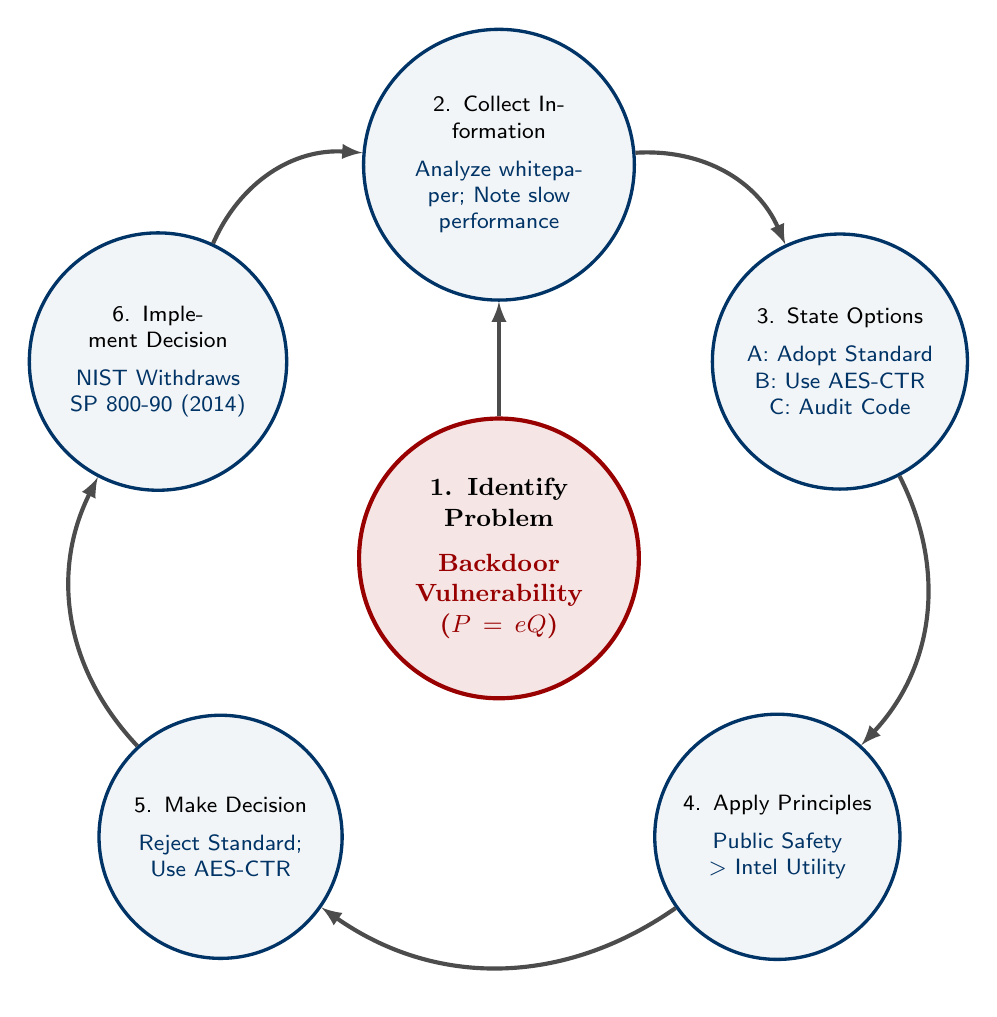
\begin{tikzpicture}
    % --- MANUAL CONFIGURATION ---
    % 1. Radius (Increase this number if circles still touch)
    \def\Radius{5} 
    
    % 2. Define colors explicitly for this diagram
    \definecolor{myBlue}{RGB}{0, 51, 102}
    \definecolor{myRed}{RGB}{153, 0, 0}
    
    % --- STYLES ---
    \tikzset{
        problemNode/.style={circle, draw=myRed, fill=myRed!10, line width=1.5pt, text width=2.5cm, align=center, font=\small\bfseries},
        stepNode/.style={circle, draw=myBlue, fill=myBlue!5, line width=1.2pt, text width=2.6cm, align=center, font=\footnotesize\sffamily},
        arrowLine/.style={-latex, draw=black!70, line width=1.5pt}
    }

    % --- NODES ---
    
    % Center Node (Problem)
    \node[problemNode] (center) at (0,0) {1. Identify Problem\\[0.5em] \textcolor{myRed}{Backdoor Vulnerability ($P=eQ$)}};

    % Outer Nodes (using polar coordinates: angle:radius)
    
    % Top (90 degrees)
    \node[stepNode] (n2) at (90:\Radius) {2. Collect Information\\[0.5em] \textcolor{myBlue}{Analyze whitepaper; Note slow performance}};

    % Top Right (30 degrees)
    \node[stepNode] (n3) at (30:\Radius) {3. State Options\\[0.5em] \textcolor{myBlue}{A: Adopt Standard\\B: Use AES-CTR\\C: Audit Code}};

    % Bottom Right (-30 degrees)
    \node[stepNode] (n4) at (-45:\Radius) {4. Apply Principles\\[0.5em] \textcolor{myBlue}{Public Safety $>$ Intel Utility}};

    % Bottom (-150 degrees)
    \node[stepNode] (n5) at (-135:\Radius) {5. Make Decision\\[0.5em] \textcolor{myBlue}{Reject Standard; Use AES-CTR}};

    % Top Left (150 degrees)
    \node[stepNode] (n6) at (150:\Radius) {6. Implement Decision\\[0.5em] \textcolor{myBlue}{NIST Withdraws SP 800-90 (2014)}};

    % --- ARROWS ---
    
    % Straight arrow center to top
    \draw[arrowLine] (center) -- (n2);

    % Cycle arrows
    \draw[arrowLine] (n2) to[bend left=35] (n3);
    \draw[arrowLine] (n3) to[bend left=35] (n4);
    \draw[arrowLine] (n4) to[bend left=35] (n5);
    \draw[arrowLine] (n5) to[bend left=35] (n6);
    \draw[arrowLine] (n6) to[bend left=35] (n2);

\end{tikzpicture}
\caption{Ethical Decision-Making Cycle Applied to the Dual\_EC\_DRBG Case}
\label{fig:ethical_cycle_dual_ec}
\end{figure}

\begin{enumerate}
    \item \textbf{Public Safety and Welfare (IEEE Code 1):} Engineers must ``hold paramount the safety, health, and welfare of the public.'' By pushing a standard known to be vulnerable, the proponents endangered the integrity of public data. As noted in the whitepaper, random-bit generation is a ``critical foundation of every security protocol''~\cite{entrust}, and compromising it puts the entire system at risk.
    
    \item \textbf{Honesty and Integrity (IEEE Code 3):} Engineers are required to be honest in stating claims. The Dual\_EC\_DRBG was presented as a secure standard despite its potential flaws. Furthermore, allegations that RSA received incentives to make it the default algorithm~\cite{entrust} suggest a breach of professional integrity and potential bribery (IEEE Code 4).
    
    \item \textbf{Technical Competence (IEEE Code 6):} The whitepaper highlights that other available algorithms were ``well-established'' and vetted by the academic community~\cite{entrust}. Dual\_EC\_DRBG was known to be inefficient (slow) compared to alternatives. Promoting an inferior technical solution for non-technical reasons violates the duty of competence.
\end{enumerate}

\subsection{Attack Path Flowchart}

\subsection{Cryptographic Integrity Spectrum}
% \begin{figure}[h]
% \centering
% \begin{tikzpicture}
%     % Draw the line
%     \draw[thick, ->] (0,0) -- (12,0);
    
%     % Ticks and Labels
%     \draw[thick] (1, 0.2) -- (1, -0.2) node[below] {\textbf{Malicious}};
%     \draw[thick] (11, 0.2) -- (11, -0.2) node[below] {\textbf{Secure}};
    
%     % Define Points
%     \node at (1, -0.7) {\small(Snake Oil)};
%     \node at (11, -0.7) {\small(Provable Security)};

%     % Point: Dual_EC_DRBG
%     \draw[red, fill=red] (3,0) circle (3pt);
%     \node[red, above] at (3,0.5) {\textbf{Dual\_EC\_DRBG}};
%     \node[text width=3cm, align=center, font=\footnotesize] at (3, -1.5) {Constructed with unknown constants; Suspect design };

%     % Point: Standard DRBG
%     \draw[blue, fill=blue] (10,0) circle (3pt);
%     \node[blue, above] at (10,0.5) {Hash\_DRBG / AES};
%     \node[text width=3cm, align=center, font=\footnotesize] at (10, -1.5) {Well-established; Academic consensus };

% \end{tikzpicture}
% \caption{Line Drawing Analysis: Integrity of Random Bit Generators}
% \label{fig:line_drawing}
% \end{figure}

\section{Conclusion}
The Dual\_EC\_DRBG case illustrates the ethical dangers of prioritizing secrecy and power over transparency and public welfare in engineering practice. Even the possibility of a backdoor in a cryptographic standard is ethically unacceptable due to the enormous reliance placed on such systems. This case emphasizes the responsibility of engineers and institutions to uphold trust, openness, and accountability, especially when their decisions affect global security infrastructure.

\bibliographystyle{plainnat}  % or another natbib style
\bibliography{mybib}     % your .bib filename without .bib


\begin{appendices}

\section{IEEE Code of Ethics}

\textbf{The Institute of Electrical and Electronics Engineers (IEEE)}

\medskip

We, the members of the IEEE, in recognition of the importance of our technologies affecting the quality of life throughout the world, and in accepting a personal obligation to our profession, its members, and the communities we serve, do hereby commit ourselves to the highest ethical and professional conduct and agree:

\begin{enumerate}
    \item to accept responsibility in making decisions consistent with the safety, health, and welfare of the public, and to disclose promptly factors that might endanger the public or the environment;
    
    \item to avoid real or perceived conflicts of interest whenever possible, and to disclose them to affected parties when they do exist;
    
    \item to be honest and realistic in stating claims or estimates based on available data;
    
    \item to reject bribery in all its forms;
    
    \item to improve the understanding of technology, its appropriate application, and potential consequences;
    
    \item to maintain and improve our technical competence and to undertake technological tasks for others only if qualified by training or experience, or after full disclosure of pertinent limitations;
    
    \item to seek, accept, and offer honest criticism of technical work, to acknowledge and correct errors, and to credit properly the contributions of others;
    
    \item to treat fairly all persons regardless of such factors as race, religion, gender, disability, age, or national origin;
    
    \item to avoid injuring others, their property, reputation, or employment by false or malicious action;
    
    \item to assist colleagues and co-workers in their professional development and to support them in following this code of ethics.
\end{enumerate}

\medskip

\noindent\textit{Approved by the IEEE Board of Directors, February 2006.}

\end{appendices}

\end{document}
%%% Local Variables: 
%%% mode: latex
%%% TeX-master: t
%%% End: 
